\documentclass[../Assignment-3-LPSMT.tex]{subfiles}
\graphicspath{{\subfix{../img/}}}

\begin{document}

\chapter{Implementazione}

Manga-check è stata sviluppata seguendo un modello a singola Activity con un
\href{https://developer.android.com/guide/navigation}{controllar di navigazione}
che funge da istanziatore e sistema di passaggio di parametri da un fragment ad un altro.\\

\section{Uso degli XML}

L'idea originale era di implementare un sistema di log in facoltativo per gli tutti gli utenti che volevano mantenere sincronizzata la propria reading list.\\
Dopo una revisione con il docente abbiamo però optato per una soluzione dall'implementazione più rapida, ovvero un importa/esporta manuale.\\
Abbiamo deciso di adottare come standard dei file salvati in locale \emph{xml}, la scelta è stata fatta per la semplicità nella verifica manuale dei dati, avendo fatto fatto largo uso della shell abd risultava molto facile verificare se il file era stato scritto in modo corretto.\\
La modificata e la gestione semplice dei file è stato possibile grazie al package \href{https://kotlinlang.org/api/latest/jvm/stdlib/org.w3c.dom/}{org.w3c.dom}, un wrapper di javascript per la gestione di elementi del DOM, che ci ha permesso di gestire ogni entry dei file \emph{xml} come un nodo con al suo interno degli attributi identificati dal nome dei campi.

\begin{center}
  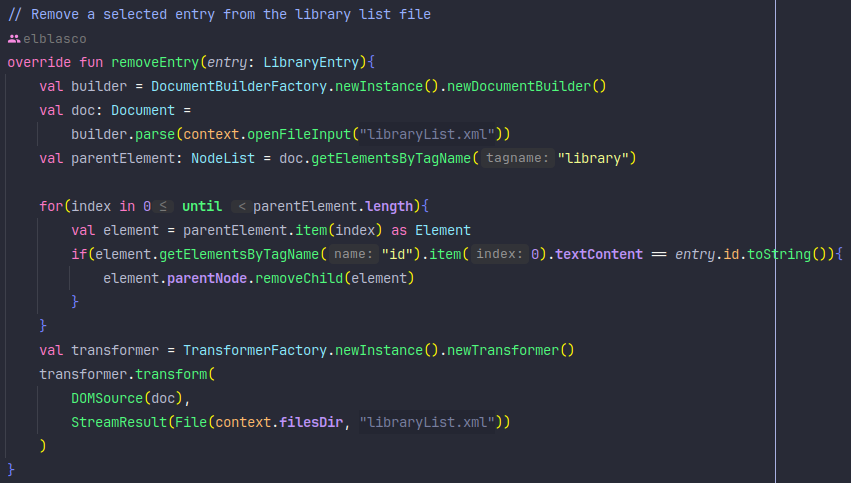
\includegraphics[scale=0.5]{removeEntry_XML.png}
  \captionof{figure}{Rimozione di una entry nella library list}
\end{center}

\section{Richieste API}

Le richieste API sono state gestite con il sopracitato package \emph{ktor}, una parte della formattazione delle rispose alle API è stata gestita lato server per ridurre il codice da scrivere nell'applicazione e non sprecare rallentare troppo l'app.\\
Per gestire le risposte al meglio abbiamo di deciso di gestire lato client come delle matrici di stringhe.\\
Nel caso sottostante riceviamo i dati come una stringa che poi viene separata grazie ad una regex ed in seguito inserita in una matrice $[n][2]$ in cui $[n][0]$ contiene l'id del manga richiesto mentre $[n][1]$ il nome.

\begin{center}
  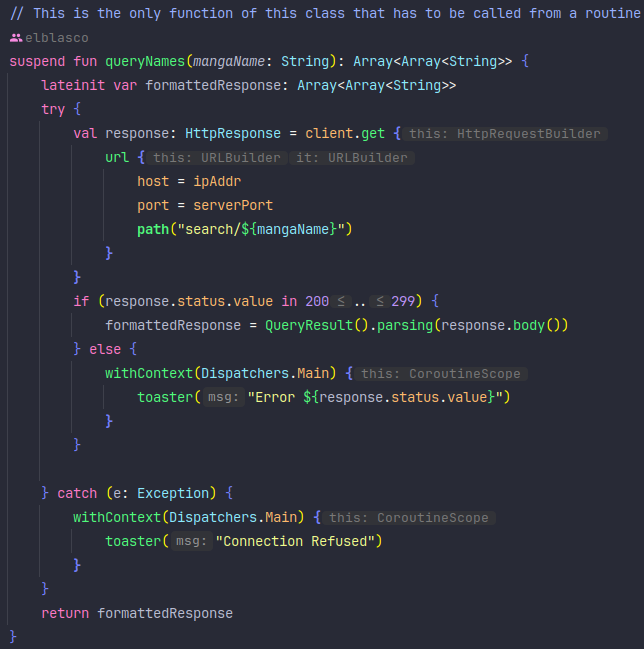
\includegraphics[scale=0.5]{queryNames.png}
  \captionof{figure}{Query dei vari nomi possibili per il manga}
\end{center}

\section{Uso di Safe Args}

Nel progetto abbiamo dovuto trasferire alcuni dati tra due fragment, come indicato nella documentazione Android abbiamo deciso di usare il \emph{navigation graph}, quindi vincolando i dati ad avere un determinato tipo.\\
Questo vincolo è stato possibile grazie all'utilizzo del plug in \href{https://developer.android.com/guide/navigation/use-graph/pass-data#Safe-args}{Safe Args} che ci ha permesso di specificare delle \emph{action} con un paylod di dati tipizzati.\\
Come descritto nelle linee guida non abbiamo passato in questi payload strutture complesse, ma solo dati di tipi primitivi come \emph{Int} e \emph{String}.

\begin{center}
  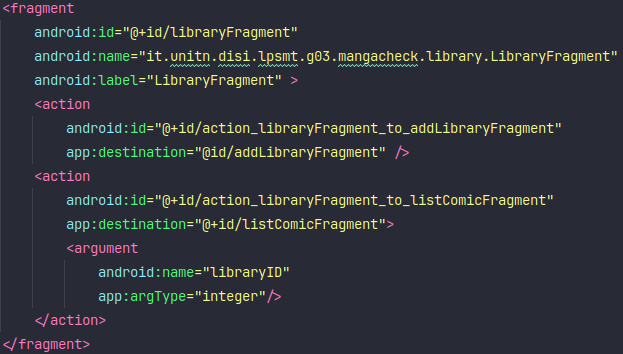
\includegraphics[scale=0.5]{action_navgraph.png}
  \captionof{figure}{Esempio di action con Safe Args}
\end{center}

\section{Backup \& Cache}

Utilizzando le \href{https://developer.android.com/guide/topics/data/autobackup}{funzionalità native} di Android abbiamo implementato un sistema di Backup che permette all'utente di spostare la reading list senza bisogno di esportare il file \emph{xml}.\\
Sfruttato la funzionalità di cache abbiamo salvato le immagini di copertina dei comic in library e reding list, ed anche una versione decompressa del file \emph{cbz} da leggere.

\section{Reader}

I \emph{cbz} vengono prima decompressi in cache, cosi da non occupare troppa RAM, una volta fatto ciò, i file vengono converti durante l'esecuzione in Bitmap ridimensionate per coprire più superficie possibile.\\
Successivamente le Bitmap vengono associate ad una ImageView che si occupa di mostrarle all'utente.\\
Nel fragment del reader abbiamo implementato anche un bottone di ricerca per navigare più agevolmente all'interno del comic e due bottoni per muoversi tra le tavole.

\end{document}
